%----------------------------------------------------------------------------------------
%	PACKAGES AND OTHER DOCUMENT CONFIGURATIONS
%----------------------------------------------------------------------------------------

\documentclass[12pt]{article}

\usepackage{polski}
\usepackage[polish]{babel}
\usepackage[utf8]{inputenc}
\usepackage{datetime}
\usepackage{graphicx}
\usepackage{tikz}
\usepackage{amsmath}
\usepackage{multirow}
\usepackage{tabularx}
\usepackage{geometry}
\geometry{
 	a4paper, 
 	left    = 20mm,
 	right	= 20mm,
 	top     = 20mm,
 	bottom  = 20mm,
}

\usetikzlibrary{arrows.meta}
 
%----------------------------------------------------------------------------------------
 
%----------------------------------------------------------------------------------------
% DATES
%----------------------------------------------------------------------------------------

\renewcommand{\dateseparator}{.}
\newdate{exercise_date}{06}{12}{2016}

%----------------------------------------------------------------------------------------

%----------------------------------------------------------------------------------------
% TIKZ PACKAGES
%----------------------------------------------------------------------------------------

\usetikzlibrary{arrows}

%----------------------------------------------------------------------------------------

\begin{document}

\begin{titlepage}

\newcommand{\HRule}{\rule{\linewidth}{0.5mm}}
% Defines a new command for the horizontal lines, change thickness here

\center
% Center everything on the page
 
%----------------------------------------------------------------------------------------
%	LOGO SECTION
%----------------------------------------------------------------------------------------


\includegraphics[width=6cm]{../res/img/logo.png}\\[1cm]
% Include a department/university logo - this will require the graphicx package
 
%----------------------------------------------------------------------------------------
 
%----------------------------------------------------------------------------------------
%	HEADING SECTIONS
%----------------------------------------------------------------------------------------

\textsc{\LARGE Akademia Górniczo-Hutnicza \\[0.2cm]
im. Stanisława Staszica w Krakowie}\\[1.5cm]
% Name of your university/college

\textsc{\Large Laboratorium problemowe}\\[0.5cm]
% Major heading such as course name

%----------------------------------------------------------------------------------------
%	TITLE SECTION
%----------------------------------------------------------------------------------------

\HRule \\[0.5cm]
{ \huge \bfseries Wahadło odwrócone}\\[0.3cm]
% Title of your document
\HRule \\[1.5cm]

\flushright
\Large \emph{Autorzy:}\\
Konrad \textsc{Adasiewcz}\\[0.1cm]  % Your name
Michał \textsc{Maciejewski}\\[0.1cm]  % Your name
% Authors

% %----------------------------------------------------------------------------------------
% %	DATE SECTION
% %----------------------------------------------------------------------------------------
% Data wykonania pracy: \\
% {\large \displaydate{exercise_date}}\\[1cm]


\vfill % Fill the rest of the page with whitespace

\end{titlepage}

\section{Model matematyczny wahadła}

Wahadło odwrócone, którego schemat znajduje się na rysunku \ref{rys:smodel},
jest systemem nieliniowym. Model obiektu został wyprowadzony z wykorzystaniem
metody \textit{Lagrange'a}. Wynikiem syntezy jest model dany równaniem
\eqref{equ:model}.

\begin{figure}[!htb] 
  \begin{center}
    \begin{tikzpicture}[scale=0.25]
  \pgfmathsetmacro{\symscale}{1}
  \pgfmathsetmacro{\segbaser}{60}
  \pgfmathsetmacro{\segbaseR}{150}
  \pgfmathsetmacro{\segmassr}{30}
  \pgfmathsetmacro{\segbasewheelr}{30}
  \pgfmathsetmacro{\segsticklen}{400}
  
  \def\segway at (#1,#2,#3){
        
    \coordinate (segbasecenter) at (#1,#2);
          
    % Draw ground
    \draw[-{Latex[length=3mm,width=2mm]}]
          (segbasecenter) ++(-\segbaseR*4 pt,-\segbaseR pt) -- 
        ++(\segbaseR*8 pt,0) node[scale=\symscale,yshift=10pt]{$x$};
    
    % Draw base
    \draw (segbasecenter) circle (\segbaser pt);
          
    % Draw engine force
    \draw[-{Latex[length=3mm,width=2mm]}]
          (segbasecenter) ++(-90pt,0) ++(-\segbaser-\segbaser*1.2 pt,0) --
          ++(\segbaser*1.2 pt,0)
          node[midway,scale=\symscale,yshift=10pt]{$f$};
          
    % Draw base friction
    \draw[-{Latex[length=3mm,width=2mm]}]
          (segbasecenter) ++(90pt,0) ++(\segbaser+\segbaser*1.2 pt,0) --
        ++(-\segbaser*1.2 pt,0)
          node[midway,scale=\symscale,yshift=10pt,xshift=5pt]{$-a\dot{x}$};
      
    % Draw base
    \draw (segbasecenter) +(-150pt,-150pt) rectangle +(150pt,150pt);
    \draw (segbasecenter) node[yshift=-25pt]{$M$};
          
    % Draw stick
    \draw (segbasecenter) ++(-#3+90:\segbaser pt)         --
          ++(-#3+90:\segsticklen pt)
          node[midway,scale=\symscale,xshift=-10pt]{$l$} ++(-#3+90:\segmassr pt)
          circle (\segmassr pt) node[scale=\symscale]{$m$};
          
    % Draw gravitational force
    \draw[-{Latex[length=3mm,width=2mm]}]
          (segbasecenter) ++(-#3+90:\segbaser + \segsticklen + \segmassr pt)
          ++(0,\segmassr + \segmassr*2 pt) -- ++(0,-\segmassr*2 pt)
          node[midway,scale=\symscale,xshift=12pt,yshift=5pt]{$mg$};
          
    % Draw stick torque
    \draw[{Latex[length=3mm,width=2mm]}-]
          (segbasecenter) ++(-#3+90:\segsticklen*0.9 pt)
          arc[radius=\segsticklen*0.9 pt,start angle=-#3+90,end angle=-#3+90+10]
          node[scale=\symscale,xshift=-5pt,yshift=12pt]{$-b\dot{\varphi}$};
          
    % Draw bearing friction
    \draw[-{Latex[length=3mm,width=2mm]}]
          (segbasecenter) ++(-#3+90-10:\segsticklen*0.9 pt)
          arc[radius=\segsticklen*0.9 pt,start angle=-#3+90-10,end angle=-#3+90]
          node[scale=\symscale,xshift=10pt,yshift=13pt]{$t$};
          
    % Draw angle base
    \draw[dashed]
          (segbasecenter) --
        ++(90:\segsticklen*1.2 pt);
          
    % Draw angle
    \draw[{Latex[length=3mm,width=2mm]}-]
          (segbasecenter) ++(-#3+90:\segsticklen*0.5 pt)
          arc[radius=\segsticklen*0.5 pt,start angle=-#3+90,end angle=90]
          node[scale=\symscale,xshift=-10pt,yshift=8pt]{$\varphi$}; 
  }
  
  \segway at (0,0,-20);
\end{tikzpicture}
    \caption{Schemat modelu wahadła}
    \label{rys:smodel} 
  \end{center}
\end{figure}

\begin{equation}
    \begin{cases}
    \ddot{x} = \frac{1}{R}\left[
    -ml^2\dot{\varphi}^2\sin{\varphi}
    +mlg\sin{\varphi}\cos{\varphi}
    -b\dot{\varphi}\cos{\varphi}
    -al\dot{x}
    +lf
    +t\cos{\varphi}\right] \\
    
    \ddot{\varphi} = \frac{1}{R}\left[
    (M+m)g\sin{\varphi}
    -ml\dot{\varphi}^2\sin{\varphi}\cos{\varphi}
    -a\dot{x}\cos{\varphi}
    -\frac{M+m}{ml}b\dot{\varphi}
    +\frac{M+m}{ml}t
    +f\cos{\varphi}\right]
    \end{cases}
    \label{equ:model}
\end{equation}

\begin{equation*}
    R = Ml + ml(1 - \cos^2{\varphi})
\end{equation*}

\newpage

\section{Identyfikacja modelu}

W celu wyznaczenia nieznanych współczynników równań modelu, przeprowadzono dwa
eksperymenty. Na podstawie odpowiedzi rzeczywistego systemu automatyczną metodą
optymalizacji parametrycznej, dobrano parametry równań tak, aby odpowiedź
modelu się z nią pokrywała.

\subsection{Eksperymenty identyfikacyjne}

\subsubsection{Wahania swobodne z zablokowanym wózkiem}

Eksperyment polegał na zablokowaniu wózka ($x = const,\dot{x} = 0,
\ddot{x} = 0$), wychyleniu wahadła z dolnego położenia równowagi
($\varphi_0=\pi$), uwolnieniu wahadła i obserwacji powstałych drgań.

Podczas identyfikacji pojawiły się znaczne rozbieżności w kształcie obwiedni
przebiegu kąta. Aby lepiej dopasować odpowiedź rzeczywistą do odpowiedzi modelu,
zmieniono charakter tarcia łożyskowania wahadła zgodnie z przekształceniem
\eqref{equ:friction}.\\

\begin{equation}
    -\frac{M+m}{ml}b\dot{\varphi} \rightarrow
    -\frac{M+m}{ml}b\tanh(s\dot{\varphi})|\dot{\varphi}|^w
    \label{equ:friction}
\end{equation}\\

Przebieg drgań wahadła oraz odpowiedź modelu przedstawiono na rysunku
\ref{rys:idf_pend1}.

\begin{figure}[!htb]
    \begin{center}
        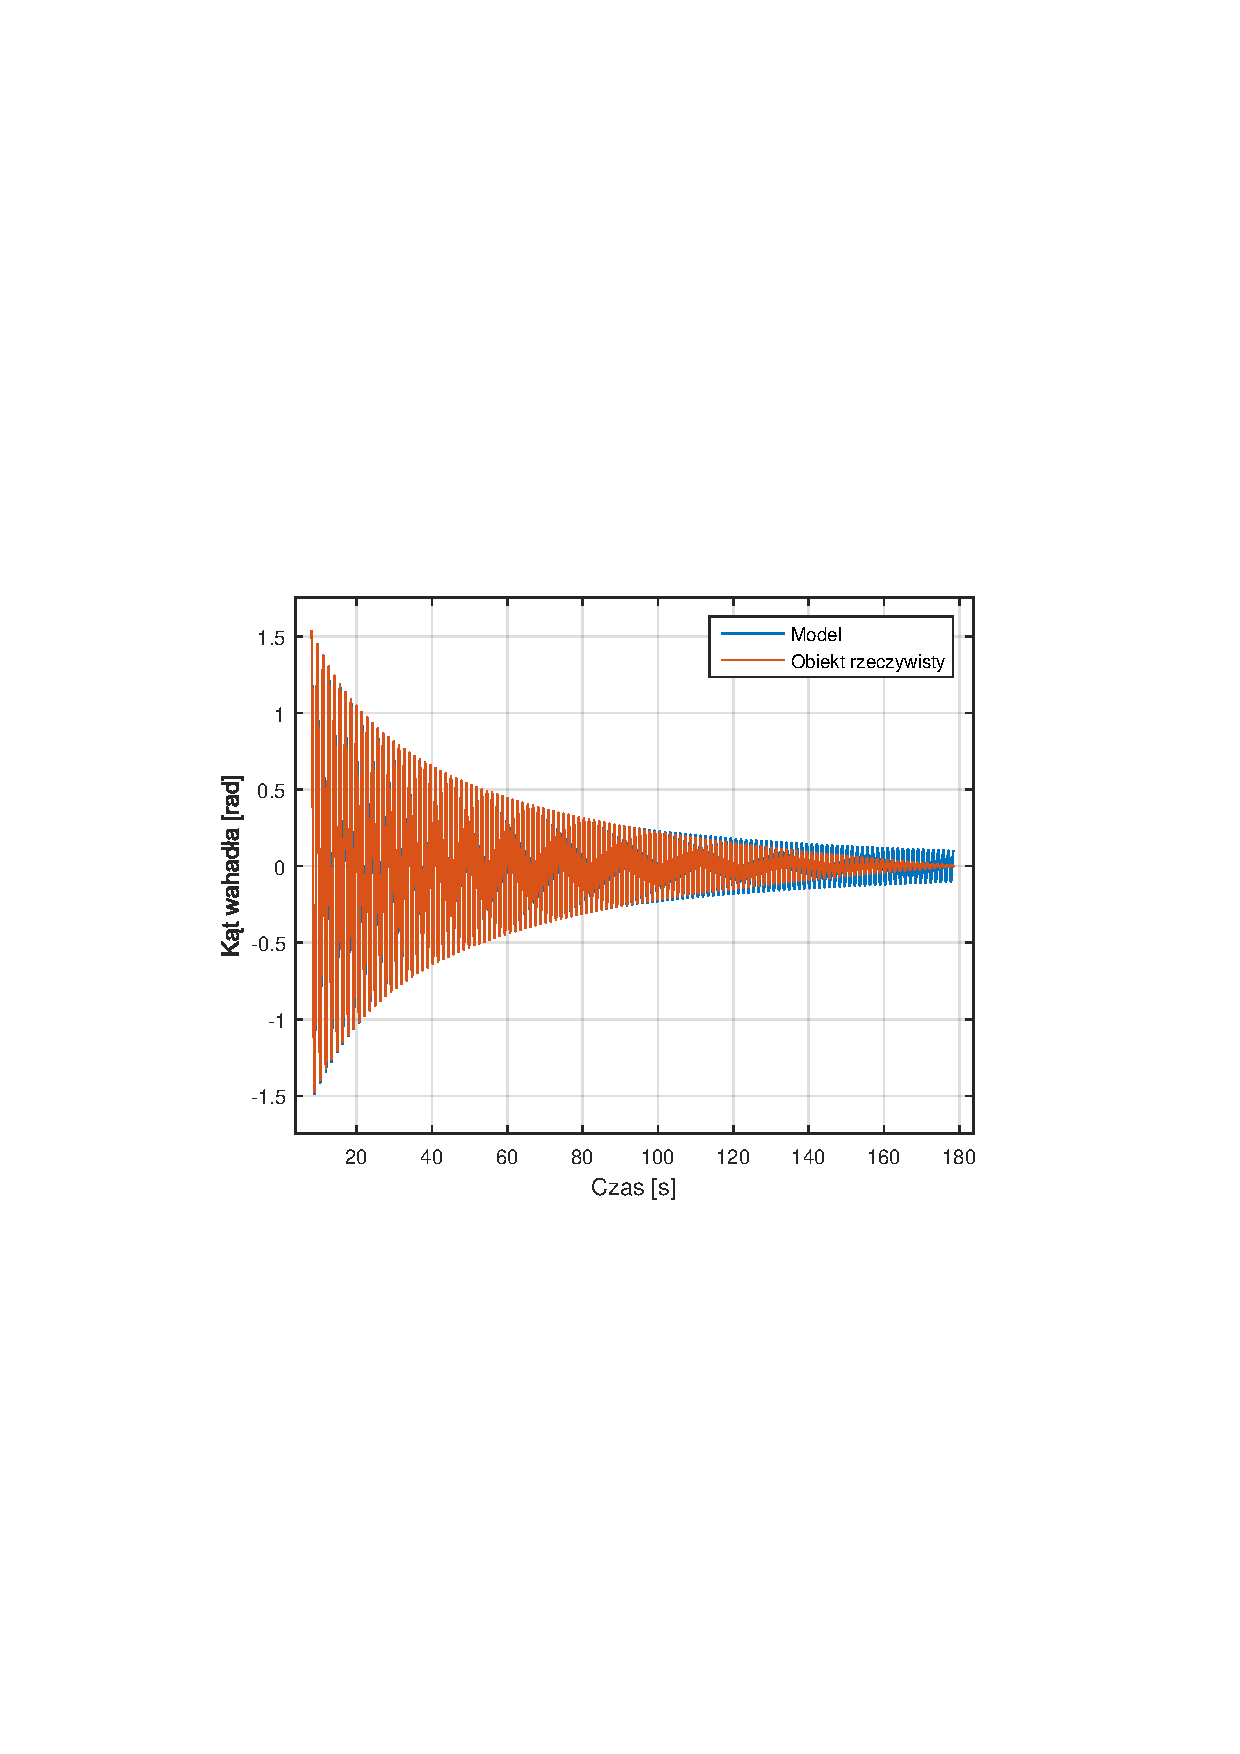
\includegraphics[width=16cm,trim=3cm 9cm 3cm 9cm,clip]
        {../res/img/idf_pend1.pdf}
    \end{center}
    \caption{Przebieg kąta wahadła w czasie dla swobodnych drgań z zablokowanym
    wózkiem} 
    \label{rys:idf_pend1}
\end{figure}

\newpage

\subsubsection{Wahania swobodne z niezablokowanym wózkiem}

W celu wyznaczenia pozostałych parametrów przeprowadzony został drugi
eksperyment. Przebiegał podobnie jak poprzedni, jednak w jego trakcie wózek nie
był zablokowany.

Przebieg drgań wahadła przedstawiono na rysunku \ref{rys:idf1_wahadlo},
pozycja wózka natomiast znajduje się na rysunku \ref{rys:idf1_wozek}.

\begin{figure}[!htb]
    \begin{center}
        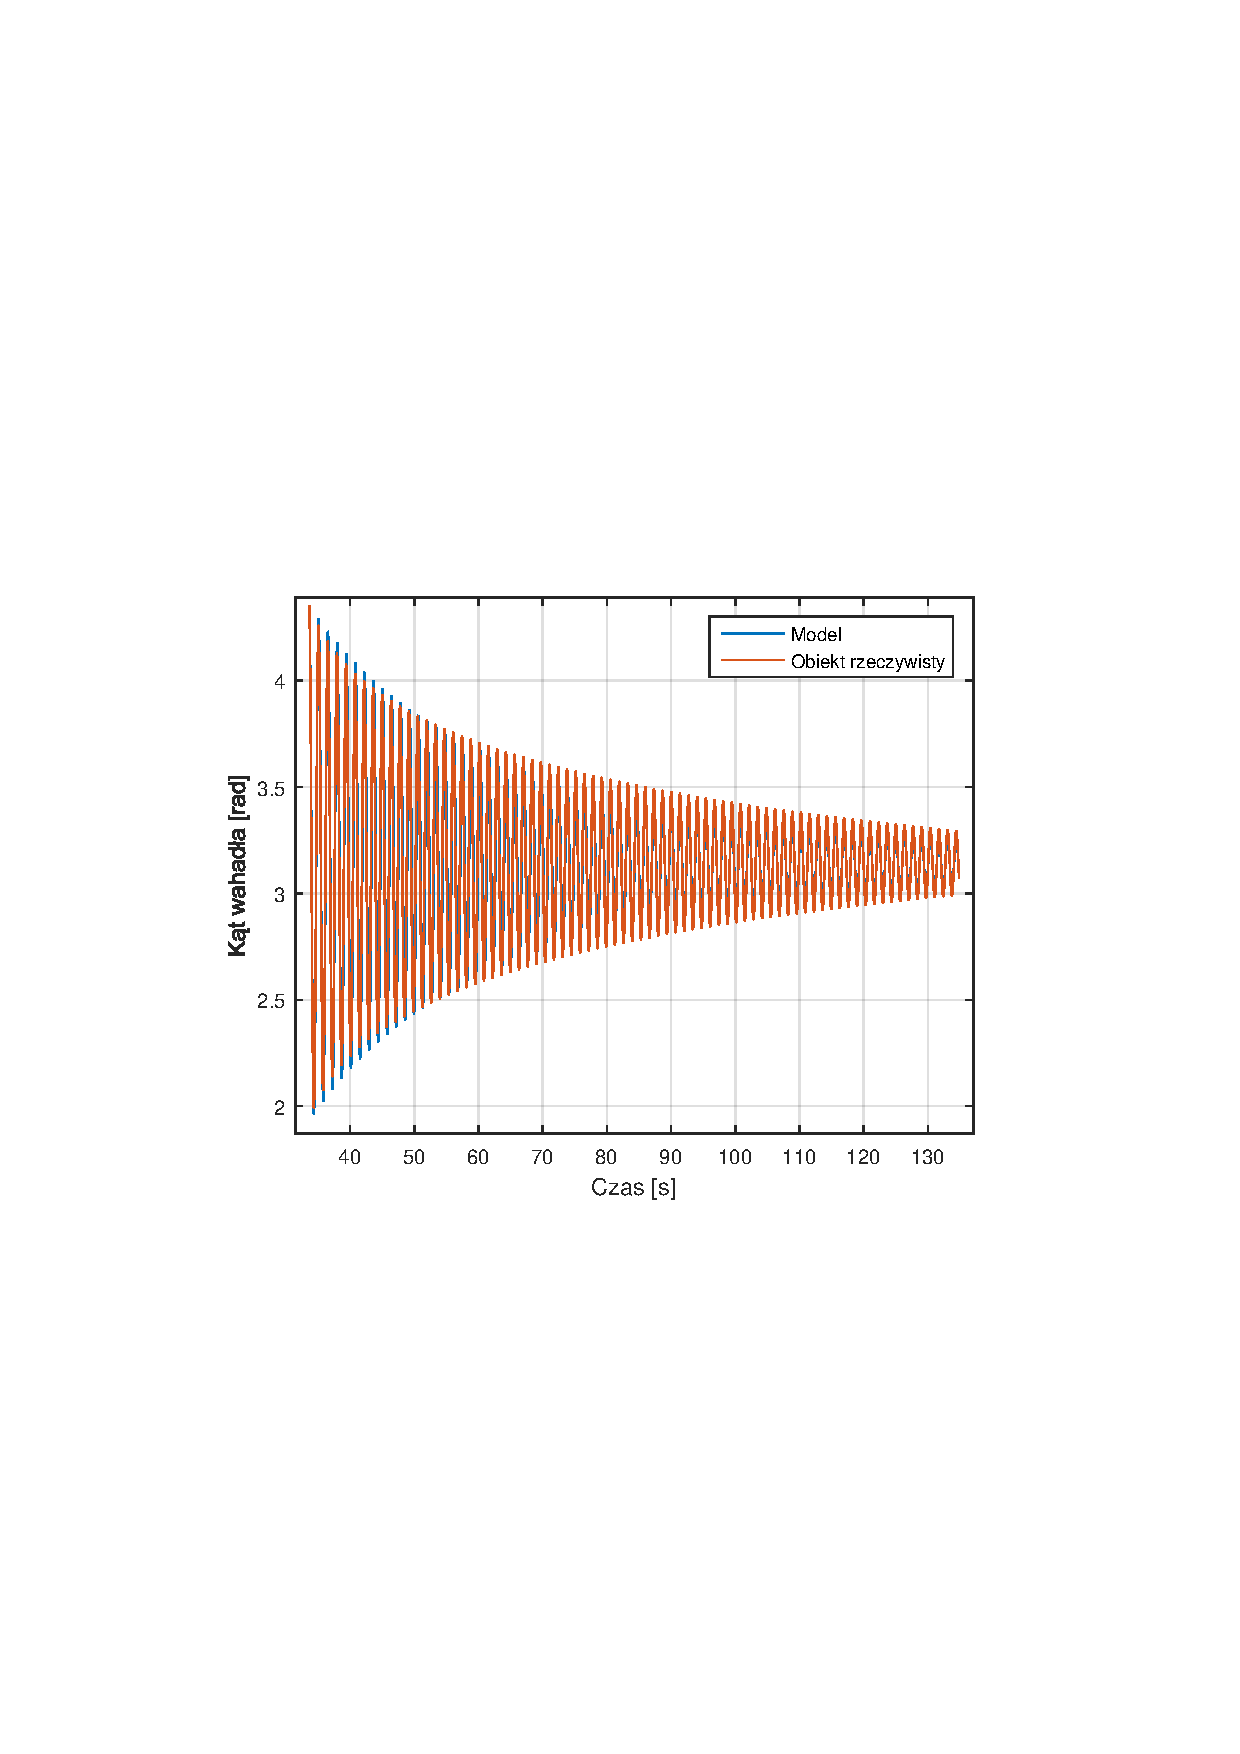
\includegraphics[width=16cm,trim=3cm 9cm 3cm 9cm,clip]
        {../res/img/idf1_wahadlo.pdf}
    \end{center}
    \caption{Przebieg kąta wahadła w czasie dla swobodnych drgań z
    niezablokowanym wózkiem} 
    \label{rys:idf1_wahadlo}
\end{figure}

\newpage

Rozbieżność spoczynkowej pozycji pomiędzy odpowiedzią rzeczywistą wózka a
odpowiedzią modelu wynika prawdopodobnie z dwóch przyczyn. Po pierwsze przyjęty
model tarcia nie odpowiada dokładnie rzeczywistemu tarciu dynamicznemu wózka,
ponadto w obiekcie rzeczywistym występuje tarcie statyczne, które z uwagi na
trudności obliczeniowe, w ogóle nie zostało uwzględnione w modelu.

\begin{figure}[!htb]
    \begin{center}
        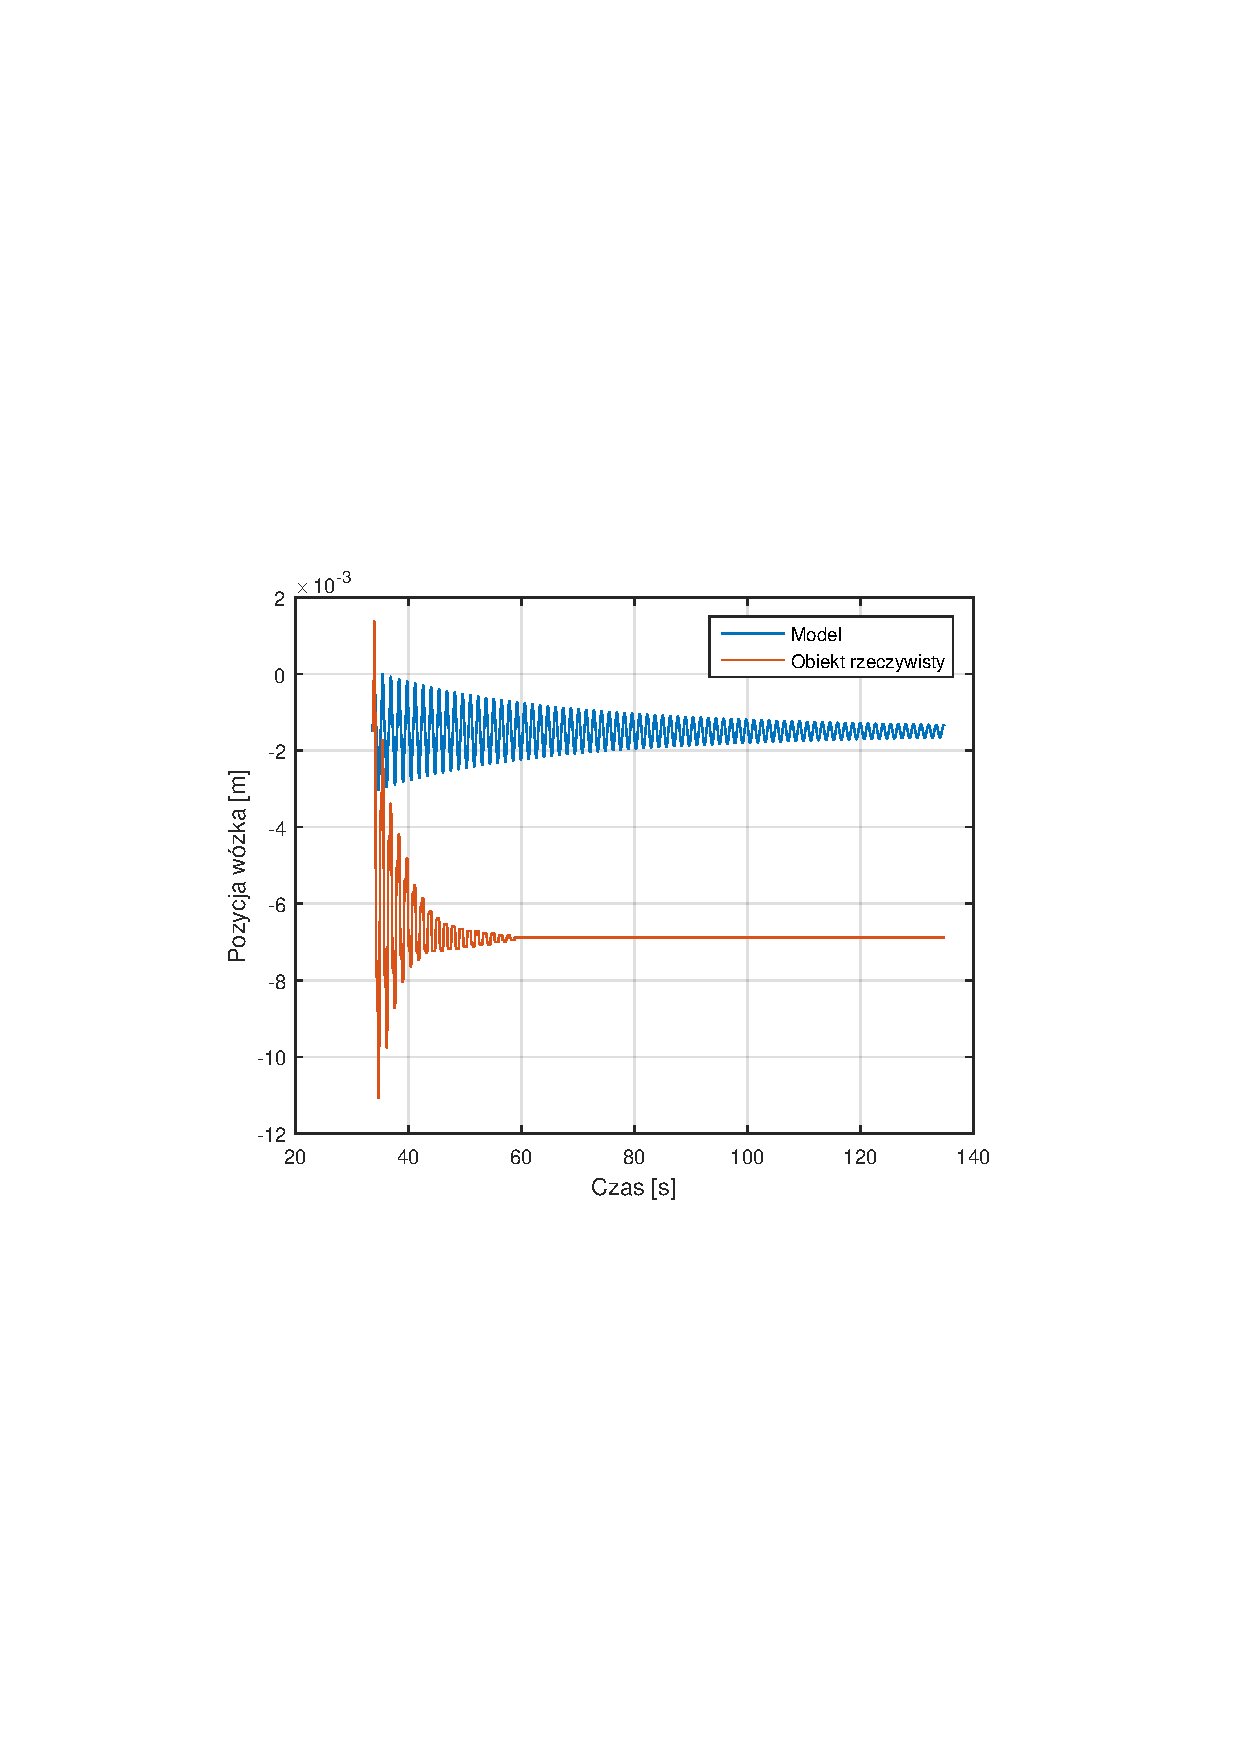
\includegraphics[width=16cm,trim=3cm 9cm 3cm 9cm,clip]
        {../res/img/idf1_wozek.pdf}
    \end{center}
    \caption{Przebieg pozycji wózka w czasie dla swobodnych drgań wahadła} 
    \label{rys:idf1_wozek}
\end{figure}

\subsection{Zidentyfikowane parametry}

Podsumowując identyfikację modelu zostały wyznaczone, zmierzone lub odczytane z
tablic parametry zamieszczone w tabeli \ref{tab:parametry}.

\begin{table}[!htb]
    \centering
    \begin{tabular}{|l|l|l|}
        \hline
        M & 0.44 & $[kg]$ \\
        m & 0.2 & $[kg]$ \\
        a & 292 & $[\frac{kg}{s}]$ \\
        b & 0.0011 & $[\frac{kg\cdot m^2}{s}]$ \\
        s & 200 & $[-]$ \\
        w & 1.5 & $[-]$ \\
        l & 0.447 & $[m]$ \\
        g & 9.81 & $[\frac{m}{s^2}]$ \\[0.01cm]
        \hline
    \end{tabular}
    \caption{Parametry modelu wyznaczone w ramach identyfikacji obiektu}
    \label{tab:parametry}
\end{table}

\newpage

\section{Regulator ciągły LQ}

Aby przeprowadzić syntezę regulatora \textit{LQ} dla badanego systemu, należy go
zlinearyzować w otoczeniu niestabilnego punktu równowagi ($\varphi = 0$). W tym
celu użyto funkcji \textit{linearize} pakietu \textrm{MATLAB}, która potrafi
zlinearyzować bloki \textrm{Simulink}-a.

W celu zweryfikowania poprawności wyznaczonego systemu zlinearyzowanego,
ręcznie wyznaczone zostały elementy macierzy $A$. Przykładowo pochodna
pierwszego równania po $\dot{x}$ to $\frac{a}{M} = 665,7$.

Macierz $A$ wyznaczona przez funkcję \textit{linearize} ma postać
\eqref{equ:amatrix}.

\begin{equation}
    A = 
    \begin{bmatrix}
        0 & 1 & 0 & 0\\
        0 & 665,7 & 4,47 & 0\\
        0 & 0 & 0 & 1\\
        0 & 1488,3 & 31,9 & 0\\
    \end{bmatrix}
    \label{equ:amatrix}
\end{equation}

Wektor wartości własnych macierzy $A$ ma postać \eqref{equ:amatrixeig1}.

\begin{equation}
    E_1 = 
    \begin{bmatrix}
              0\\
      -665,6797\\
        -4,6757\\
         4,6907\\
    \end{bmatrix}
    \label{equ:amatrixeig1}
\end{equation}

Dla takiego problemu regulator LQ gwarantuje sterowanie optymalne względem
wskaźnika jakości \eqref{equ:wskjak}.

\begin{equation}
    q = \int_{-\infty}^{\infty}(xQx^T + uRu^T)
    \label{equ:wskjak}
\end{equation}

W celu wyznaczenia macierzy $K$ regulatora LQ przyjęto następujące macierze $Q$
i $R$.

\begin{equation}
    Q = 
    \begin{bmatrix}
        0,1 & 0 & 0 & 0\\
        0 & 0,001 & 0 & 0\\
        0 & 0 & 1 & 0\\
        0 & 0 & 0 & 1\\
    \end{bmatrix}
    \label{equ:lqq}
\end{equation}

\begin{equation}
    R = 0,00001
    \label{equ:lqr}
\end{equation}

Taka macierz $Q$ kładzie nacisk na zminimalizowanie wychylenia i prędkości
wahadła, trochę mniejszy priorytet ma pozycja wózka, natomiast nie przykłada się
do minimalizacji prędkości wózka, która sam w sobie jest stabilna. Macierze
zostały dobrane na podstawie obserwacji wektora wartości własnych macierzy A,
oraz zdrowego rozsądku.

Taki system z zamkniętą pętlą sprzężenia zwrotnego, posiada wektor wartości
własnych \eqref{equ:amatrixeig2}.

\begin{equation}
    E_1 = 
    \begin{bmatrix}
      -1742,6\\
      -2,4 + 1,5i\\
      -2,4 - 1,5i\\
      -0,3\\
    \end{bmatrix}
    \label{equ:amatrixeig2}
\end{equation}

Zatem układ zamknięty będzie stabilny.

\newpage

Na rysunku \ref{rys:lq_response_model} widoczna jest odpowiedź modelu
startującego z niezerowego wychylenia początkowego wahadła.

\begin{figure}[!htb]
    \begin{center}
        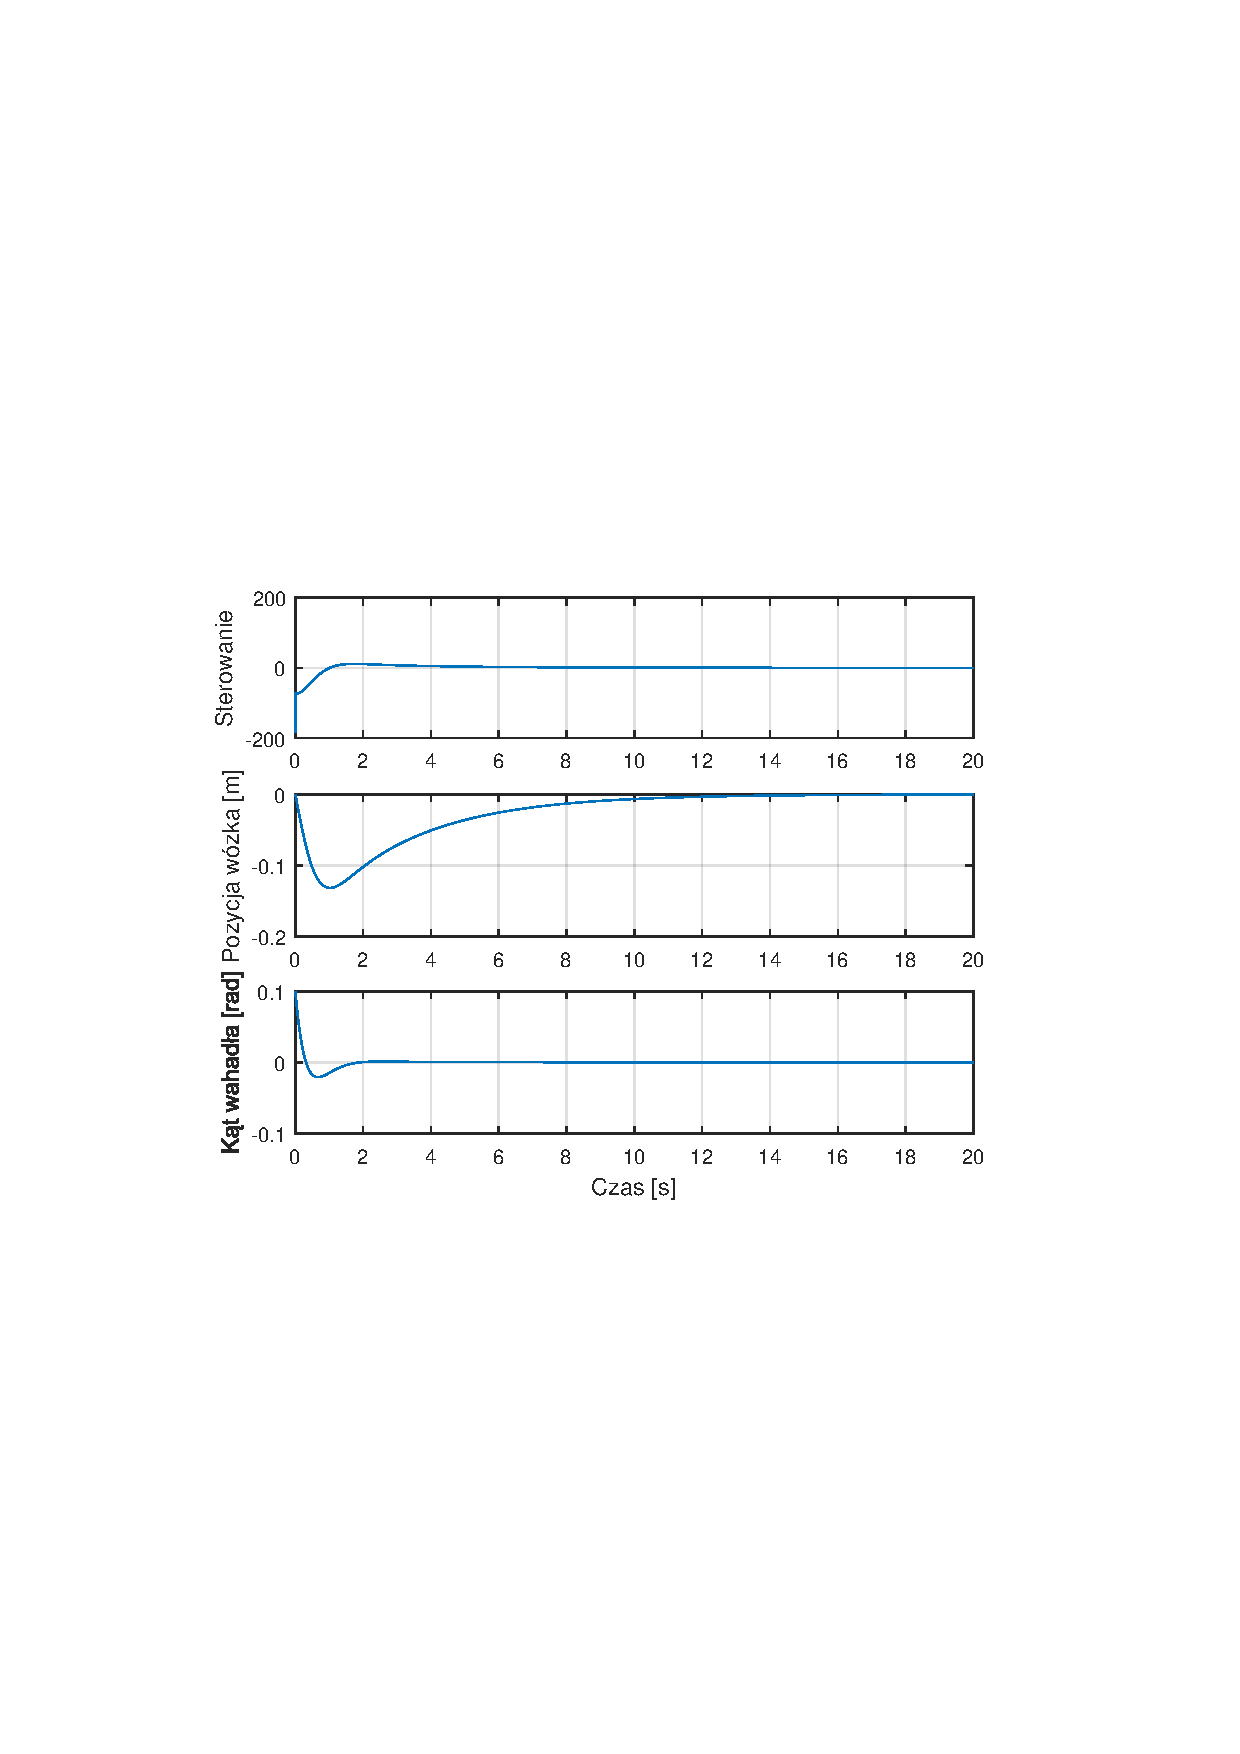
\includegraphics[width=16cm,trim=3cm 9cm 3cm 9cm,clip]
        {../res/img/lq_response_model.pdf}
    \end{center}
    \caption{Sterowanie i stan modelu w czasowej odpowiedzi regulowanego
    systemu}
    \label{rys:lq_response_model}
\end{figure}



\end{document}